\documentclass{beamer}

% Scelta del tema
\usetheme{Madrid}
\usecolortheme{default}

% Pacchetti standard
\usepackage[utf8]{inputenc}
\usepackage[italian]{babel}
\usepackage{graphicx}

% Informazioni sul Titolo
\title[Sky Analytics Engine]{Sky Analytics Engine}
\subtitle{Analisi batch e Metriche del Traffico Aereo}
\author[Simonelli, Masci]{Flavio Simonelli \and Francesco Masci}
\institute[SABD]{
    Corso Architettura e Sistemi per Big Data\\
    Corso di Laurea Magistrale in Ingegneria Informatica\\
    Università di Roma "Tor Vergata"
}
\date[12 Giugno 2026]{12 Giugno 2026}

\titlegraphic{
\includegraphics[width=2cm]{logos/logo_tor_vergata.png}}

\begin{document}

% Slide del Titolo
\begin{frame}
    \titlepage
\end{frame}

% Slide dell'Indice
\begin{frame}{Indice}
    \tableofcontents[hideallsubsections]
\end{frame}

% Big Data Stack
\section{Big Data Stack}
\begin{frame}{Big Data Stack}
    \centering
    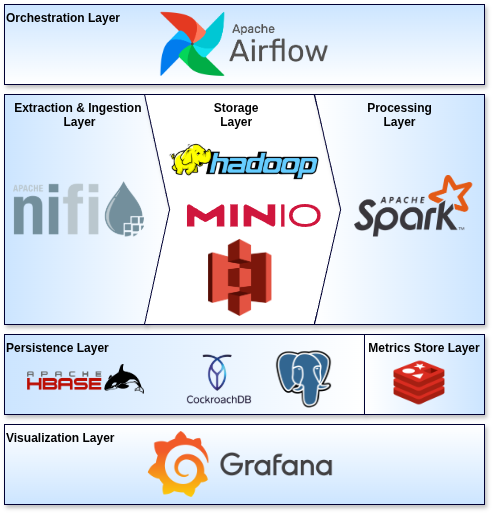
\includegraphics[width=\textwidth,height=0.85\textheight,keepaspectratio]{../Report/graphs/BigDataStack.png}
\end{frame}

% Flow diagram
\section{Flow Diagram}
\begin{frame}{Flow Diagram}
    \centering
    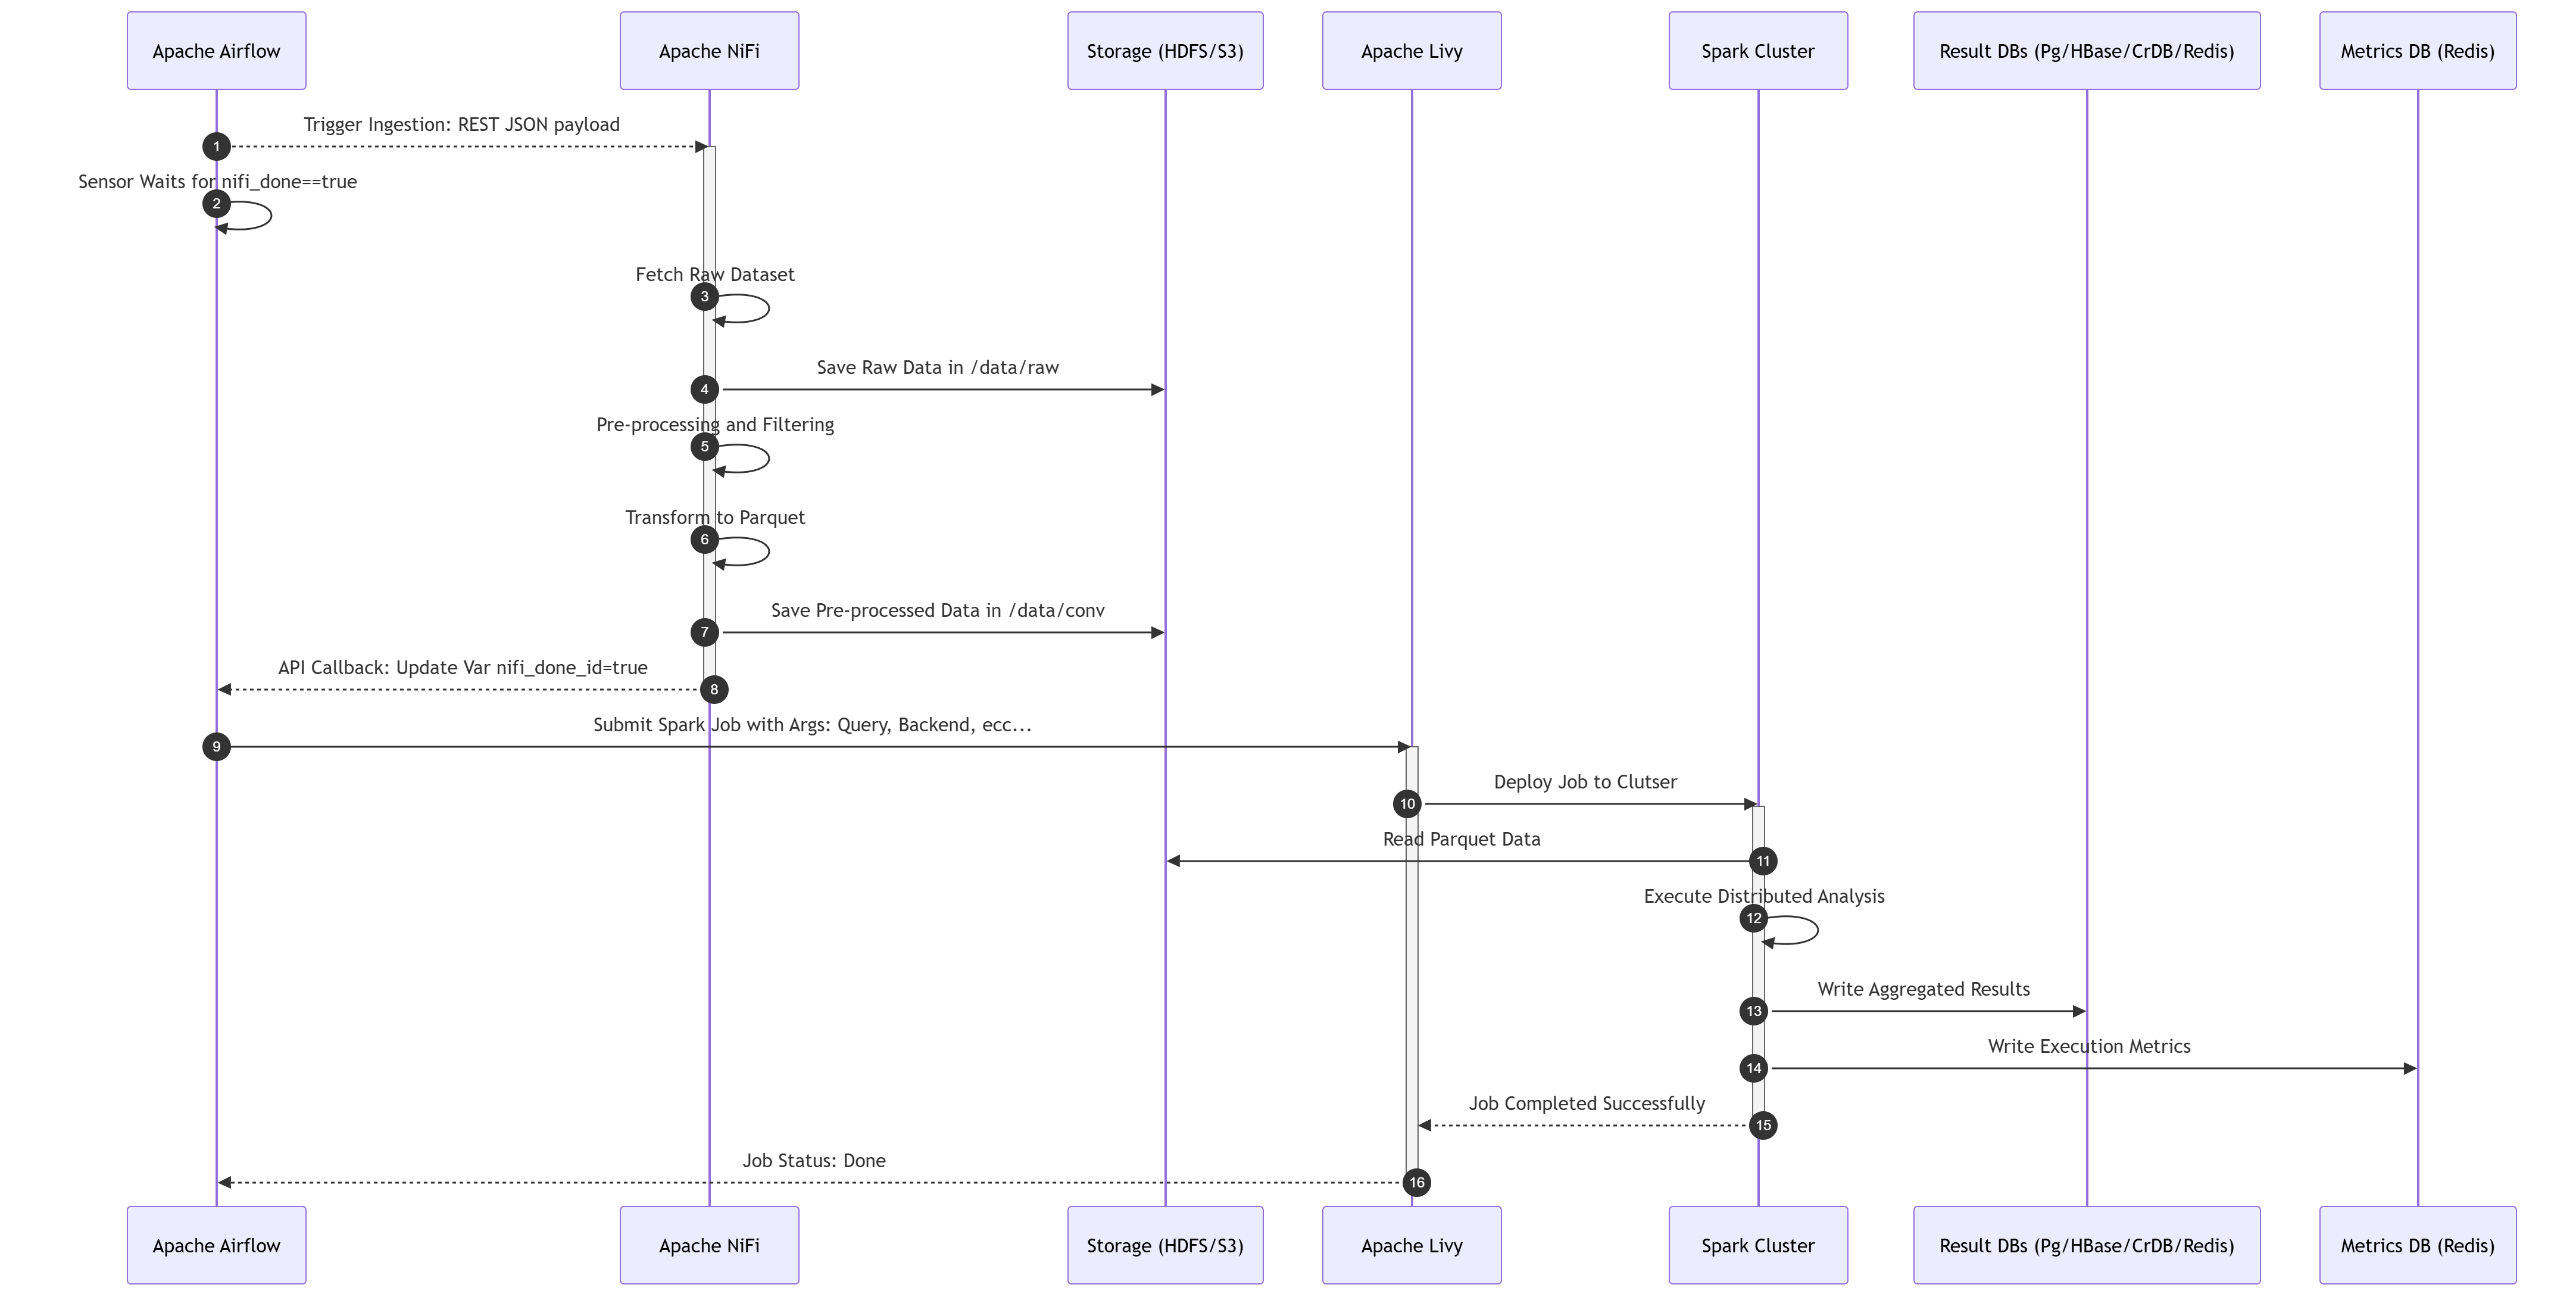
\includegraphics[width=\textwidth,height=0.85\textheight,keepaspectratio]{../Report/graphs/sequence_diagram.png}
\end{frame}

% Deployment
\section{Deployment}
\begin{frame}{Deployment}
    \begin{columns}[T]
        \column{0.48\textwidth}
        \centering
        \textbf{EC2 Deployment}
        \vfill
        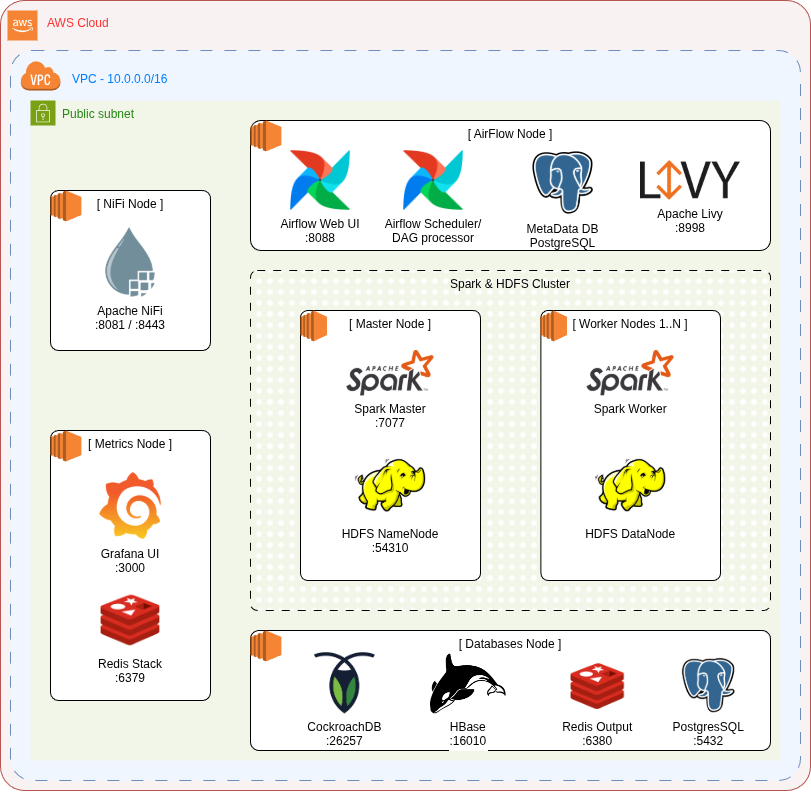
\includegraphics[width=\linewidth,height=0.6\textheight,keepaspectratio]{../Report/graphs/DeploymentView.png}
        
        \column{0.48\textwidth}
        \centering
        \textbf{EMR Deployment}
        \vfill
        \begin{center}
            \Large [Immagine in arrivo]
        \end{center}
    \end{columns}
\end{frame}

% Data Extraction & Ingestion
\section{Data Extraction \& Ingestion}

\begin{frame}{Architettura Event-Driven della Pipeline NiFi}
    \begin{itemize}
        \item \textbf{Panoramica}: Il flusso SAE\_Ingestion\_Pipeline è modulare e orchestrato esternamente tramite Apache Airflow.
        \item \textbf{Innesco Dinamico}: La pipeline è data-driven. Si avvia con un payload JSON da cui estrae configurazioni vitali:
        \begin{itemize}
            \item Run ID ed Expected SHA-1
            \item Percorsi e tipologia di storage
            \item URL di callback
        \end{itemize}
        \item \textbf{Ruolo}: NiFi funge da middleware intelligente tra la sorgente dei dati e il Data Lake.
    \end{itemize}
\end{frame}

\begin{frame}{Estrazione, Validazione e Smistamento Iniziale}
    \begin{itemize}
        \item \textbf{Unpacking \& Integrità}: I dati compressi vengono scompattati. Un check crittografico confronta l'hash SHA-1 con quello atteso per prevenire corruzioni.
        \item \textbf{Routing Logico}: Separazione del flusso principale (voli) dai file di supporto (dizionari) per evitare congestioni.
        \item \textbf{Filtraggio Preliminare}: Selezione dei soli file target (es. file \texttt{ONTIME\_REPORTING}) scartando i dati non pertinenti.
    \end{itemize}
\end{frame}

\begin{frame}{Biforcazione: Salvataggio Raw e Inoltro al Processing}
    \begin{itemize}
        \item \textbf{Lo Split Logico}: Dopo la validazione e il filtraggio, il flusso si sdoppia seguendo il pattern Data Lake.
        \item \textbf{Percorso A - Raw Data Storage}: I dati grezzi vengono salvati. Il sistema di destinazione (HDFS o S3) è deciso dinamicamente in base ai parametri del payload iniziale.
        \item \textbf{Percorso B - Verso la Trasformazione}: Una copia viene instradata verso i moduli successivi per il filtraggio a livello di record e la conversione per l'analisi.
    \end{itemize}
\end{frame}

\begin{frame}{Trasformazione e Ottimizzazione in Parquet}
    \begin{itemize}
        \item \textbf{Merge \& Compattazione}: I dati CSV vengono accorpati per prevenire lo "Small Files Problem" penalizzante nei sistemi distribuiti.
        \item \textbf{Conversione Parquet}: Conversione dei record nel formato colonnare Parquet, riducendo lo spazio e velocizzando le query analitiche.
        \item \textbf{Preparazione per Spark}: Iniezione di attributi di ottimizzazione (\texttt{PARTITION\_PRUNING}, \texttt{PREDICATE\_PUSHDOWN}) per guidare l'engine di calcolo.
    \end{itemize}
\end{frame}

\begin{frame}{Storage Finale e Chiusura del Ciclo}
    \begin{itemize}
        \item \textbf{Salvataggio Processed Data}: I file Parquet vengono salvati nello strato Silver del Data Lake, pronti per l'analisi.
        \item \textbf{Chiusura (Finish\_AirFlow)}: NiFi notifica il completamento dell'ingestion tramite chiamata HTTP all'URL di callback.
        \item \textbf{Orchestrazione}: Il segnale di successo (o errore) sblocca Airflow, permettendo l'avvio automatico dei successivi job di calcolo distribuito (Spark).
    \end{itemize}
\end{frame}

\end{document}
